\section{Hasil untuk total perdagangan Indonesia}\label{sec:aggregate}
\subsection{Bukti long run masih belum cukup}
Model total Indonesia memakai ekspor ke seluruh negara dan impor dari seluruh negara. Sampel utamanya berisi 61 kuartal, yaitu 2011Q1--2026Q1.

ARDL memilih lag $(2,3,0,4)$. Urutannya adalah rasio perdagangan, GDP Indonesia, aktivitas luar negeri, dan kurs. NARDL memilih $(2,0,3,0,4)$, dengan dua angka terakhir untuk partial sums apresiasi dan depresiasi. Ini pilihan AIC dari kandidat yang tersedia, bukan kepastian bahwa proses ekonomi mempunyai lag persis seperti itu.

\begin{table}[!htbp]\centering\caption{Bounds test untuk total perdagangan Indonesia}
{\small\setlength{\tabcolsep}{3pt}\renewcommand{\arraystretch}{1.15}
\begin{tabular}{p{0.1\linewidth}p{0.08\linewidth}p{0.08\linewidth}p{0.1\linewidth}p{0.1\linewidth}p{0.12\linewidth}p{0.22\linewidth}}
\toprule
\textbf{Model} & \textbf{F} & \textbf{t} & \textbf{p F(I1)} & \textbf{p t(I1)} & \textbf{p joint-X} & \textbf{Keputusan}\\
\midrule
ARDL & 2,481 & -2,280 & 0,369 & 0,434 & 0,259 & No rejection\\
NARDL & 3,799 & -2,887 & 0,094 & 0,279 & 0,011 & Inconclusive\\
\bottomrule
\end{tabular}
}\label{tab:worldbounds}
\end{table}

Pada ARDL, koefisien kurs sekitar 0,429 dengan p-value 0,661. Confidence interval melewati nol, dan bounds test belum mendukung hubungan long run. Diagnostic tests tidak menemukan masalah pada pemeriksaan yang dipakai, tetapi itu belum mengubah hasil bounds test.

Pada NARDL, koefisien depresiasi sekitar 2,572 dengan p-value 0,040. Koefisien apresiasi sekitar $-2,142$, sedangkan p-value uji asymmetry sekitar 0,006. Jika hanya angka ini yang dilihat, hasilnya tampak mendukung perbaikan saat rupiah melemah.

Tetapi p-value upper bound untuk F sekitar 0,094 dan untuk t sekitar 0,279. Keduanya belum memenuhi aturan utama 5\%. CUSUMSQ juga memberi catatan stabilitas. Jadi, signifikansi satu koefisien belum cukup untuk menyimpulkan adanya hubungan long run yang kuat.

\begin{figure}[!htbp]\centering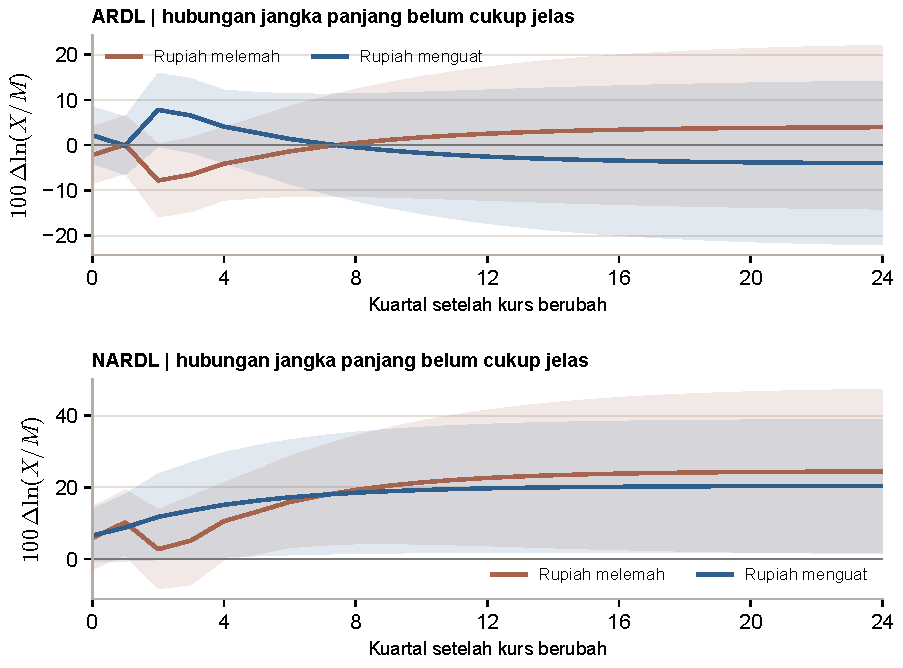
\includegraphics[width=\linewidth]{assets/response_WORLD.pdf}
\caption{Respons total perdagangan Indonesia. Cokelat: rupiah melemah; biru: rupiah menguat. Area berwarna adalah confidence interval 95\% per horizon. Positif berarti rasio ekspor/impor membaik.}\label{fig:world}
\end{figure}

\subsection{Apa yang bisa dibaca dari grafik?}
Garis utama ARDL memburuk dahulu lalu membaik. Tetapi confidence interval-nya cukup lebar dan masih mencakup nol pada bagian penting jalur. NARDL lebih banyak mengarah pada perbaikan, dengan fluktuasi pada awal periode.

Grafik membantu memahami jalur yang dihasilkan model. Namun bentuk yang terlihat baik belum menyelesaikan masalah pada bounds test dan stabilitas. Model utama masih belum memberikan dasar long run yang kuat.

Pada NARDL, kedua arah kurs bisa sama-sama terlihat memperbaiki rasio. Ini muncul dari tanda koefisien apresiasi dan depresiasi. Hasil tersebut belum bisa dibaca sebagai saran bahwa rupiah menguat maupun melemah pasti sama-sama menguntungkan. Model merangkum pengalaman historis dan perubahan lain yang bergerak bersama kurs.

Baseline mulai 2010 dipakai agar bisa dibandingkan dengan run sebelumnya. Data mulai 2006 juga dijalankan sebagai robustness check. Kita tidak memilih periode hanya karena tandanya lebih sesuai harapan.

\subsection{Contoh: apa arti koefisien 3,356?}
Contoh Australia lebih mudah dipakai karena NARDL-nya lolos pemeriksaan utama. Koefisien depresiasinya $\widehat{\beta}_-=\AusBetaMath$. Jika perubahan log kurs sebesar $-\ln(1.10)$, respons long run yang ditampilkan adalah
\begin{equation}
 -100\,\widehat{\beta}_-\big[-\ln(1.10)\big]\simeq\AusResponseMath.
\end{equation}
Angka \AusResponse{} adalah \textbf{poin log kali seratus}, bukan kenaikan surplus dolar sebesar \AusResponse\%. Untuk mengubahnya menjadi perubahan persentase rasio ekspor/impor, rumusnya:
\begin{equation}
 100\left[\exp\{-\widehat{\beta}_-\delta^-\}-1\right].
\end{equation}
Hasilnya sekitar \AusRatioPct\%. Ini tetap perubahan rasio ekspor/impor yang dihitung dari model. Angkanya belum berarti ekspor naik \AusRatioPct\% dan belum menjadi ramalan kebijakan yang pasti.

Koefisien, poin log, persentase rasio, dan perubahan surplus dolar adalah empat hal yang berbeda. Semuanya tetap bergantung pada asumsi dan ketidakpastian model asalnya.
